%\section{Tapered waveguide}
%tapered_waveguide
Tapered waveguide is inhomogeneous waveguide on shape, whose dimensions in the tapered section changes slowly along the longitude dirccetion\cite{linear_tapered_waveguides}. Tapered structure enables the waveguide to receive more light so that improve the coupling efficiency between beam source and waveguide.  
The author of \cite{design_fabrication_tapered_waveguide} has presented two general types of tapered waveguide: conventional taper like Fig. \ref{fig:conventional_taper} and inverse taper like Fig. \ref{fig:inverse_taper}. For a conventional taper the entry is wider than the exit while for an inverse taper the entry is narrower than the exit. In this section the conventional taper will be discussed
\begin{figure}[!ht]
\centering
%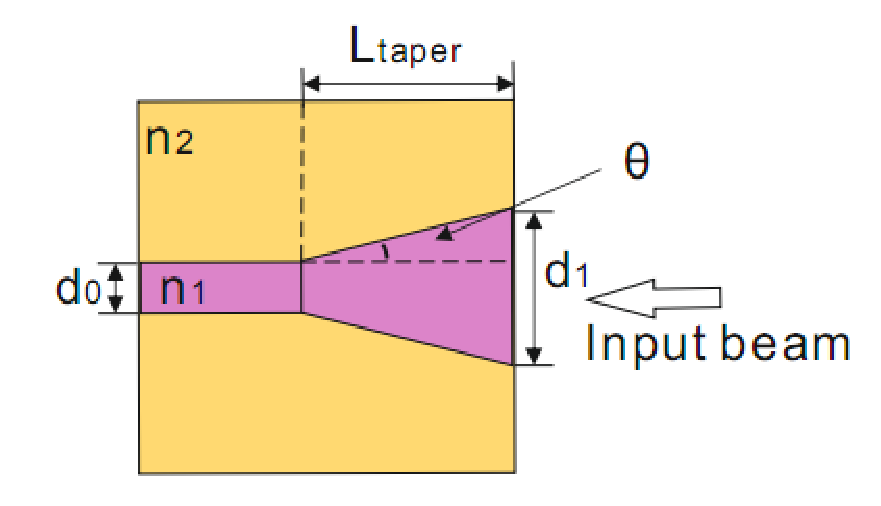
\includegraphics[width=0.7\textwidth]{bilder/convernational_taper}
\caption{Schema of the conventional taper.}
\label{fig:conventional_taper}
\end{figure}
\begin{figure}[!ht]
\centering
%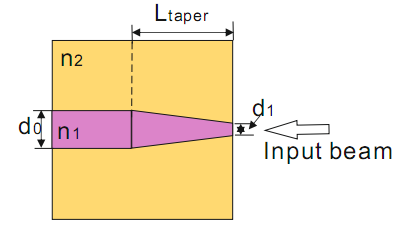
\includegraphics[width=0.7\textwidth]{bilder/inverse_taper}
\caption{Schema of the inverse taper.}
\label{fig:inverse_taper}
\end{figure}

.
Two properties, the width of a taper interface and the taper angle, of the taper may strongly affect the coupling efficiency. For convenient calculations simulations are running due to variations of taper width and taper length respectively.
